\documentclass{article}
\usepackage[preprint]{neurips_2024}
\usepackage[utf8]{inputenc}
\usepackage[T1]{fontenc}
\usepackage[colorlinks=true,linkcolor=black,citecolor=blue!50!black,urlcolor=blue!50!black]{hyperref}
\usepackage{url}
\usepackage{booktabs}
\usepackage{amsmath,amssymb,amsthm}
\usepackage{cancel}
\usepackage{microtype}
\usepackage{xcolor}
\usepackage{tikz}
\usetikzlibrary{arrows.meta,positioning}

\newtheorem{proposition}{Proposition}[section]
\newtheorem{lemma}[proposition]{Lemma}
\newtheorem{corollary}[proposition]{Corollary}
\theoremstyle{definition}
\newtheorem{definition}[proposition]{Definition}
\newtheorem{assumption}{Assumption}
\newtheorem{example}[proposition]{Example}
\theoremstyle{remark}
\newtheorem{remark}[proposition]{Remark}

\newcommand{\E}{\mathbb{E}}
\newcommand{\dE}{\Delta E}
\newcommand{\dP}{\Delta P}
\newcommand{\Ob}{\bar O}
\newcommand{\KL}{\mathrm{KL}}
\newcommand{\Cov}{\mathrm{Cov}}

\title{The State Defect, Plasticity, Empowerment and the Return}

\author{XXX}

\begin{document}
\maketitle

\begin{abstract}
We study an agent whose policy reads a memory that is a recursive function of its history, in an environment on which we make no assumption. The state defect is the information the history carries about the next observation beyond the memory and the action. We split it into four terms by the chain rule, show that two of them are the memory's errors about the agent's one-step empowerment and plasticity, write the defect over time as a sum over the memory updates, and relate it exactly to the error of a critic that reads the memory. We then take an objective that combines the return with predictive information and derive conditions for the best policy and the best memory. Every statement is followed by its proof.
\end{abstract}

\section{Introduction}

A small agent in a large world keeps a memory $M_t$ that is much smaller than its history $h_t$ and acts on the memory alone. We ask how the information the memory drops affects the agent's prediction of what it will see, its own decisions, and its return, and what the memory should keep when the agent pursues the return. We make no assumption on the environment and only two on the agent: the memory is updated recursively, and the policy reads the memory.

The note is built from the bottom up, and each section uses only what comes before it.
\begin{itemize}
\item Section~\ref{sec:setting} fixes the setting and the notation, which is not changed later, and proves two lemmas that the rest of the note uses.
\item Section~\ref{sec:terms} defines the state defect $D_t$ and its four terms $D^0_t$, $\dE_t$, $\dP_t$, $D^+_t$, and shows that $\dE_t$ and $\dP_t$ are the memory's errors about one-step empowerment and plasticity.
\item Section~\ref{sec:time} writes the defect over time as a sum, over the memory updates, of the information each update discards.
\item Section~\ref{sec:value} relates the defect to the error of a critic that reads the memory, first by exact identities and then by bounds.
\item Section~\ref{sec:objective} takes an objective that combines the return with predictive information and derives conditions for the best policy and the best memory.
\item Section~\ref{sec:reward} separates the reward inside the four terms. No other section depends on it.
\item Section~\ref{sec:known} lists which statements are known, which follow directly from known results, and which we did not find in the literature, and states open questions.
\end{itemize}

We checked every identity in the note, and the stationarity conditions of Section~\ref{sec:objective} by finite differences, on small random environments in which the law of the next observation depends on the whole history, by computing the exact law of all trajectories. The largest error is below $10^{-12}$ for the identities and below $10^{-7}$ for the finite differences. The script is \texttt{checks/verify\_note.py} in the repository, and each check is labelled by the statement it tests.

\section{Setting, notation and two lemmas}\label{sec:setting}

\subsection{Setting}

\begin{center}
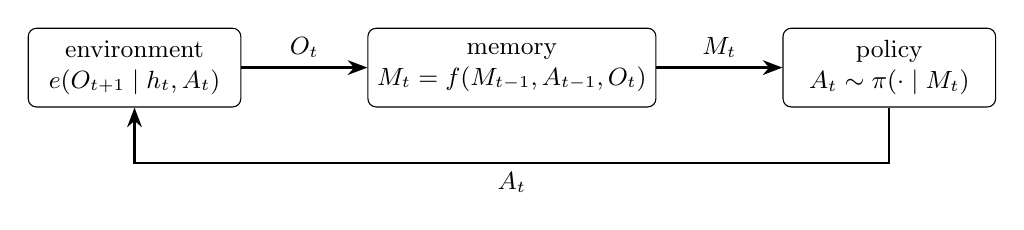
\begin{tikzpicture}[>={Stealth[length=2.5mm]}, node distance=10mm and 16mm,
  box/.style={draw, rounded corners=3pt, minimum height=10mm, minimum width=27mm, align=center, font=\small}]
\node[box] (world) {environment\\ $e(O_{t+1}\mid h_t, A_t)$};
\node[box, right=of world] (mem) {memory\\ $M_t = f(M_{t-1}, A_{t-1}, O_t)$};
\node[box, right=of mem] (pol) {policy\\ $A_t \sim \pi(\cdot \mid M_t)$};
\draw[->, thick] (world) -- node[above, font=\small] {$O_t$} (mem);
\draw[->, thick] (mem) -- node[above, font=\small] {$M_t$} (pol);
\draw[->, thick] (pol.south) -- ++(0,-7mm) -| node[pos=0.25, below, font=\small] {$A_t$} (world.south);
\end{tikzpicture}
\end{center}

At each step $t=1,2,\dots$ the agent sees an observation $O_t=(R_t,\Ob_t)$, which contains the reward $R_t$ and the rest of the observation $\Ob_t$, and takes an action $A_t$. All sets are finite, and the rewards lie in an interval of length $\Delta R$. We make three assumptions.

\begin{assumption}[Environment]\label{as:env}
The next observation may depend on the whole history: $O_{t+1}\sim e(\cdot\mid h_t,A_t)$. No Markov or stationarity condition is imposed.
\end{assumption}

\begin{assumption}[Memory]\label{as:mem}
The memory is updated recursively by a fixed map, $M_1=f_1(O_1)$ and $M_{t+1}=f(M_t,A_t,O_{t+1})$, so $M_t$ is a function of $h_t$.
\end{assumption}

\begin{assumption}[Policy]\label{as:pol}
The policy depends on the history only through the memory: $P(A_t=a\mid h_t)=\pi(a\mid M_t)$.
\end{assumption}

All probabilities, entropies and mutual informations are taken under the law of the agent's own experience, and logarithms are natural.

\subsection{Notation}

\begin{center}
\small
\begin{tabular}{p{0.2\linewidth}p{0.72\linewidth}}
\toprule
symbol & meaning\\
\midrule
$h_t$ & the history $(O_1,A_1,\dots,A_{t-1},O_t)$\\
$M_t$ & the memory at $t$ (Assumption~\ref{as:mem})\\
$U_t$ & $(M_{t-1},A_{t-1},O_t)$, the input of the update that produces $M_t=f(U_t)$; $U_1=O_1$\\
$Y_{t,k}$ & $(M_t,A_t,O_{t+1},\dots,A_{t+k-1},O_{t+k})$, the memory at $t$ extended by what the agent did and saw up to $O_{t+k}$; $Y_{t,0}=M_t$\\
$Z_{t,k}$ & $(Y_{t,k},A_{t+k})$, the same with the action $A_{t+k}$; $Z_{t,0}=(M_t,A_t)$\\
$G_t$ & $\sum_{k\ge0}\gamma^kR_{t+k+1}$, the return, with $\gamma\in(0,1)$\\
$q_\pi(h,a)$, $v_\pi(h)$ & $\E[G_t\mid h_t=h,A_t=a]$ and $\E[G_t\mid h_t=h]$\\
$q_\pi(m,a)$, $v_\pi(m)$ & $\E[G_t\mid M_t=m,A_t=a]$ and $\E[G_t\mid M_t=m]$, at the time $t$ of the context\\
$D_t$, $D^0_t$, $\dE_t$, $\dP_t$, $D^+_t$ & the state defect and its four terms (Definition~\ref{def:terms})\\
$D_{t,k}$, $D^0_{t,k}$, \dots & the same terms for the extended memory (Definition~\ref{def:ext})\\
\bottomrule
\end{tabular}
\end{center}

$Y_{t,k}$ is a function of $h_{t+k}$, and $M_{t+k}$ is a function of $Y_{t,k}$, by applying $f$ $k$ times. The history $h_{t+k}$ and the pair $(h_t,Y_{t,k})$ determine each other.

\subsection{Facts from information theory}

We use the following standard facts \citep[Ch.~2]{cover2006elements}.
\begin{enumerate}
\item[(H1)] $I(X;Y\mid Z)=H(X\mid Z)-H(X\mid Y,Z)=I(Y;X\mid Z)$.
\item[(H2)] The chain rule: $H(X,Y\mid Z)=H(X\mid Z)+H(Y\mid X,Z)$ and $I(X;Y,W\mid Z)=I(X;Y\mid Z)+I(X;W\mid Y,Z)$.
\item[(H3)] $I(X;Y\mid Z)\ge0$, with equality exactly when $X$ and $Y$ are independent given $Z$.
\item[(H4)] If $W$ is a function of $X$, then $I(X;Y\mid Z)=I(X,W;Y\mid Z)$, and conditioning on $(X,W)$ is the same as conditioning on $X$.
\end{enumerate}
By (H1) and (H4), every quantity of the form $I(h_t;X\mid M_t,V)$ in this note is
\begin{equation}\label{eq:star}
I(h_t;X\mid M_t,V)=H(X\mid M_t,V)-H(X\mid h_t,V),
\end{equation}
the uncertainty about $X$ given the memory minus the uncertainty given the history, both given $V$. The co-information of $X,Y,W$ given $Z$ is $I(X;Y;W\mid Z)=I(X;Y\mid Z)-I(X;Y\mid Z,W)$. It is symmetric in $X,Y,W$, by (H2) applied to $I(X;Y,W\mid Z)$ in two orders, and it can be negative.

\subsection{Two lemmas}

\begin{lemma}[The action depends on the past only through the memory]\label{lem:action}
Let $n\ge1$, let $C$ be a function of $h_n$ that determines $M_n$, and let $X$ be a function of $h_n$. Then $A_n$ and $X$ are independent given $C$, so $I(X;A_n\mid C)=0$.
\end{lemma}

\begin{proof}
By Assumption~\ref{as:pol}, $P(A_n=a\mid h_n)=\pi(a\mid M_n)$. Since $(X,C)$ is a function of $h_n$, $P(A_n=a\mid X,C)=\E[\pi(a\mid M_n)\mid X,C]=\pi(a\mid M_n)$, because $M_n$ is a function of $C$. The same argument with $C$ alone gives $P(A_n=a\mid C)=\pi(a\mid M_n)$. The two conditional laws agree, which is the independence; (H3) gives the zero.
\end{proof}

We use three cases: $I(h_t;A_t\mid M_t)=0$ (with $n=t$, $C=M_t$); $I(h_t;A_{t+1}\mid M_t,A_t,O_{t+1})=0$ (with $n=t+1$ and $C=(M_t,A_t,O_{t+1})$, which determines $M_{t+1}$); and $I(X;A_{s+k}\mid Y_{s,k})=0$ for $X=h_s$ or $X=U_s$ (with $n=s+k$ and $C=Y_{s,k}$).

\begin{lemma}[What each update discards]\label{lem:updates}
For $n\ge1$ and any variables $X$ and $V$,
\[
I(h_n;X\mid M_n,V)=\sum_{s=1}^{n}I(U_s;X\mid Y_{s,n-s},V).
\]
Grouping the updates up to $t$ and after $t$, for $1\le t\le n$,
\[
I(h_n;X\mid M_n,V)=I(Y_{t,n-t};X\mid M_n,V)+I(h_t;X\mid Y_{t,n-t},V).
\]
\end{lemma}

\begin{proof}
Write $Y_{0,n}=h_n$. For $1\le s\le n$ two facts hold.
\begin{enumerate}
\item[(i)] $Y_{s,n-s}$ is a function of $Y_{s-1,n-s+1}$. For $s\ge2$, $Y_{s-1,n-s+1}=(U_s,A_s,O_{s+1},\dots,O_n)$ and $Y_{s,n-s}=(f(U_s),A_s,O_{s+1},\dots,O_n)$. For $s=1$, $Y_{1,n-1}=(f_1(O_1),A_1,O_2,\dots,O_n)$ is a function of $h_n$.
\item[(ii)] Given $Y_{s,n-s}$, the variables $Y_{s-1,n-s+1}$ and $U_s$ determine each other: $U_s$ is part of $Y_{s-1,n-s+1}$, and $Y_{s-1,n-s+1}$ is $U_s$ followed by $(A_s,O_{s+1},\dots,O_n)$, which are part of $Y_{s,n-s}$.
\end{enumerate}
By (i), (H4) and (H2), $I(Y_{s-1,n-s+1};X\mid V)=I(Y_{s,n-s};X\mid V)+I(Y_{s-1,n-s+1};X\mid Y_{s,n-s},V)$, and by (ii) the last term is $I(U_s;X\mid Y_{s,n-s},V)$. Hence
\[
I(Y_{s-1,n-s+1};X\mid V)-I(Y_{s,n-s};X\mid V)=I(U_s;X\mid Y_{s,n-s},V).
\]
Summing over $s=1,\dots,n$, the left side telescopes to $I(h_n;X\mid V)-I(M_n;X\mid V)$, which is $I(h_n;X\mid M_n,V)$ by (H2) and (H4), because $M_n$ is a function of $h_n$. Summing only over $s\le t$ gives $I(h_n;X\mid V)-I(Y_{t,n-t};X\mid V)=I(h_n;X\mid Y_{t,n-t},V)=I(h_t;X\mid Y_{t,n-t},V)$, since given $Y_{t,n-t}$ the history $h_n$ and $h_t$ determine each other; summing over $s>t$ gives $I(Y_{t,n-t};X\mid V)-I(M_n;X\mid V)=I(Y_{t,n-t};X\mid M_n,V)$.
\end{proof}

In words: the information the history carries about $X$ beyond the memory is the sum, over the memory updates so far, of the information each update removed from its input, counted as far as the observations and actions after it have not restored it.

\section{The state defect and its four terms}\label{sec:terms}

\begin{definition}[The state defect and its four terms]\label{def:terms}
The state defect and its four terms are the following conditional mutual informations.
\begin{center}
\small
\begin{tabular}{llll}
\toprule
term & definition & what is predicted & what is given (besides $M_t$ or $h_t$)\\
\midrule
$D_t$ & $I(h_t;O_{t+1}\mid M_t,A_t)$ & next observation & action\\
$D^0_t$ & $I(h_t;O_{t+1}\mid M_t)$ & next observation & nothing\\
$\dE_t$ & $I(h_t;A_t\mid M_t,O_{t+1})$ & action & next observation\\
$\dP_t$ & $I(h_t;A_{t+1}\mid M_t,A_t)$ & next action & action\\
$D^+_t$ & $I(h_t;O_{t+1}\mid M_t,A_t,A_{t+1})$ & next observation & both actions\\
\bottomrule
\end{tabular}
\end{center}
By \eqref{eq:star}, each term is how much better the history predicts the variable in the third column than the memory does, given the variables in the fourth column. In particular $D_t=\E\big[\log\big(P(O_{t+1}\mid h_t,A_t)/P(O_{t+1}\mid M_t,A_t)\big)\big]$.
\end{definition}

\begin{proposition}[Three orders of one chain rule]\label{prop:orders3}
Under Assumptions~\ref{as:mem} and~\ref{as:pol}, the chain rule (H2) expands $I(h_t;A_t,O_{t+1},A_{t+1}\mid M_t)$ as
\begin{align*}
&\text{in the order of time }(A_t,O_{t+1},A_{t+1}): && 0+D_t+0,\\
&\text{in the order }(O_{t+1},A_t,A_{t+1}): && D^0_t+\dE_t+0,\\
&\text{in the order }(A_t,A_{t+1},O_{t+1}): && 0+\dP_t+D^+_t.
\end{align*}
Hence $D_t=D^0_t+\dE_t=\dP_t+D^+_t$, and all five quantities are nonnegative.
\end{proposition}

\begin{proof}
In the three orders, the terms are, respectively,
\begin{align*}
&I(h_t;A_t\mid M_t)+I(h_t;O_{t+1}\mid M_t,A_t)+I(h_t;A_{t+1}\mid M_t,A_t,O_{t+1}),\\
&I(h_t;O_{t+1}\mid M_t)+I(h_t;A_t\mid M_t,O_{t+1})+I(h_t;A_{t+1}\mid M_t,O_{t+1},A_t),\\
&I(h_t;A_t\mid M_t)+I(h_t;A_{t+1}\mid M_t,A_t)+I(h_t;O_{t+1}\mid M_t,A_t,A_{t+1}).
\end{align*}
$I(h_t;A_t\mid M_t)=0$ and $I(h_t;A_{t+1}\mid M_t,A_t,O_{t+1})=0$ by Lemma~\ref{lem:action}; the other terms are those of Definition~\ref{def:terms}. The three expansions are equal, and each term is nonnegative by (H3).
\end{proof}

In words: both splits read one action out of the order of time. The first reads $A_t$ after the observation it produced, and the second reads $A_{t+1}$ before the observation it responds to. In the order of time the actions add nothing, because the policy reads only the memory.

\begin{definition}[One-step empowerment and plasticity]\label{def:EP}
Following the one-step form of \citet{abel2025plasticity}, the empowerment of the action and the plasticity of the next action, computed from the history and from the memory, are
\begin{gather*}
E_t=I(A_t;O_{t+1}\mid h_t),\qquad E_t(M)=I(A_t;O_{t+1}\mid M_t),\\
P_{t+1}=I(O_{t+1};A_{t+1}\mid h_t,A_t),\qquad P_{t+1}(M)=I(O_{t+1};A_{t+1}\mid M_t,A_t).
\end{gather*}
\end{definition}

\begin{proposition}[$\dE_t$ and $\dP_t$ are the memory's errors]\label{prop:mismatch}
Under Assumptions~\ref{as:mem} and~\ref{as:pol}:
\begin{enumerate}
\item[(a)] $\dE_t=E_t-E_t(M)$ and $\dP_t=P_{t+1}(M)-P_{t+1}$;
\item[(b)] $H(A_t\mid M_t)=E_t(M)+\dE_t+H(A_t\mid h_t,O_{t+1})$;
\item[(c)] $I(M_{t+1};A_{t+1})=I(M_t,A_t;A_{t+1})+P_{t+1}+\dP_t$, and $I(M_t,A_t;A_{t+1})+\dP_t=I(h_t,A_t;A_{t+1})$.
\end{enumerate}
\end{proposition}

\begin{proof}
(a) By (H1),
\begin{align*}
E_t-E_t(M)
&=\big[\cancel{H(A_t\mid h_t)}-H(A_t\mid h_t,O_{t+1})\big]\\
&\quad-\big[\cancel{H(A_t\mid M_t)}-H(A_t\mid M_t,O_{t+1})\big]\\
&=H(A_t\mid M_t,O_{t+1})-H(A_t\mid h_t,O_{t+1})=\dE_t,
\end{align*}
where the cancelled entropies are equal by Lemma~\ref{lem:action} and the last step is \eqref{eq:star}. Similarly,
\begin{align*}
P_{t+1}(M)-P_{t+1}
&=\big[H(A_{t+1}\mid M_t,A_t)-\cancel{H(A_{t+1}\mid M_t,A_t,O_{t+1})}\big]\\
&\quad-\big[H(A_{t+1}\mid h_t,A_t)-\cancel{H(A_{t+1}\mid h_t,A_t,O_{t+1})}\big]\\
&=H(A_{t+1}\mid M_t,A_t)-H(A_{t+1}\mid h_t,A_t)=\dP_t,
\end{align*}
where the cancelled entropies are equal by Lemma~\ref{lem:action}.

(b) $H(A_t\mid M_t)=H(A_t\mid h_t)$ by Lemma~\ref{lem:action}, and by (H1) $H(A_t\mid h_t)=I(A_t;O_{t+1}\mid h_t)+H(A_t\mid h_t,O_{t+1})=E_t+H(A_t\mid h_t,O_{t+1})$. Insert $E_t=E_t(M)+\dE_t$ from (a).

(c) $A_{t+1}$ depends on $(M_t,A_t,O_{t+1})$ only through $M_{t+1}=f(M_t,A_t,O_{t+1})$, so $I(M_{t+1};A_{t+1})=I(M_t,A_t,O_{t+1};A_{t+1})$. By (H2),
\begin{align*}
I(M_t,A_t,O_{t+1};A_{t+1})&=I(M_t,A_t;A_{t+1})+I(O_{t+1};A_{t+1}\mid M_t,A_t)\\
&=I(M_t,A_t;A_{t+1})+P_{t+1}(M),
\end{align*}
and $P_{t+1}(M)=P_{t+1}+\dP_t$ by (a). For the second identity, (H2) and (H4) give $I(h_t,A_t;A_{t+1})=I(M_t,A_t;A_{t+1})+I(h_t;A_{t+1}\mid M_t,A_t)$, and the last term is $\dP_t$.
\end{proof}

\begin{corollary}\label{cor:mismatch}
$\dE_t\le H(A_t\mid M_t)$, so $\dE_t=0$ when the policy is deterministic. $\dP_t\le P_{t+1}(M)\le I(M_{t+1};A_{t+1})$, so $\dP_t=0$ when $A_{t+1}$ does not depend on $O_{t+1}$ given $(M_t,A_t)$.
\end{corollary}

\begin{proof}
Every other term in Proposition~\ref{prop:mismatch}(b) and (c) is nonnegative.
\end{proof}

In words: a memory that merges histories underestimates how much the agent's action influences the next observation, by $\dE_t$, and overestimates how much its next action responds to that observation, by $\dP_t$. The randomness of the policy limits the first, and the information the next decision uses limits the second.

The next definition applies the four terms to the memory at $t$ extended by what came after it. Sections~\ref{sec:time} and~\ref{sec:value} use it.

\begin{definition}[The four terms of the extended memory]\label{def:ext}
For $k\ge0$,
\begin{gather*}
D_{t,k}=I(h_t;O_{t+k+1}\mid Z_{t,k}),\qquad D^0_{t,k}=I(h_t;O_{t+k+1}\mid Y_{t,k}),\\
\dE_{t,k}=I(h_t;A_{t+k}\mid Y_{t,k},O_{t+k+1}),\qquad \dP_{t,k}=I(h_t;A_{t+k+1}\mid Z_{t,k}),\\
D^+_{t,k}=I(h_t;O_{t+k+1}\mid Z_{t,k},A_{t+k+1}).
\end{gather*}
They are the terms of Definition~\ref{def:terms} at time $t+k$, with $h_t$ in place of $h_{t+k}$ and the extended memory in place of $M_{t+k}$. For $k=0$ they are $D_t,D^0_t,\dE_t,\dP_t,D^+_t$.
\end{definition}

\begin{proposition}\label{prop:ext}
Under Assumptions~\ref{as:mem} and~\ref{as:pol}:
\begin{enumerate}
\item[(a)] $D_{t,k}=D^0_{t,k}+\dE_{t,k}=\dP_{t,k}+D^+_{t,k}$;
\item[(b)] $D_{t,k}\le D_{t+k}$, $D^0_{t,k}\le D^0_{t+k}$, $\dE_{t,k}\le\dE_{t+k}$, $\dP_{t,k}\le\dP_{t+k}$ and $D^+_{t,k}\le D^+_{t+k}$.
\end{enumerate}
\end{proposition}

\begin{proof}
(a) As in Proposition~\ref{prop:orders3}, expand $I(h_t;A_{t+k},O_{t+k+1}\mid Y_{t,k})$ and $I(h_t;O_{t+k+1},A_{t+k+1}\mid Z_{t,k})$ in two orders each. The terms $I(h_t;A_{t+k}\mid Y_{t,k})$ and $I(h_t;A_{t+k+1}\mid Y_{t,k+1})$, with $Y_{t,k+1}=(Z_{t,k},O_{t+k+1})$, are zero by Lemma~\ref{lem:action}.

(b) By the second identity of Lemma~\ref{lem:updates} with $n=t+k$, $I(h_{t+k};X\mid M_{t+k},V)\ge I(h_t;X\mid Y_{t,k},V)$, since the first term there is nonnegative. Take $(X,V)$ equal to $(O_{t+k+1},A_{t+k})$, $(O_{t+k+1},\text{nothing})$, $(A_{t+k},O_{t+k+1})$, $(A_{t+k+1},A_{t+k})$ and $(O_{t+k+1},(A_{t+k},A_{t+k+1}))$.
\end{proof}

\section{The defect over time}\label{sec:time}

\begin{proposition}[Each update discards information about later observations]\label{prop:charge}
Under Assumptions~\ref{as:mem} and~\ref{as:pol}:
\begin{enumerate}
\item[(a)] $D_n=\sum_{s=1}^{n}I(U_s;O_{n+1}\mid Z_{s,n-s})$ for every $n\ge1$;
\item[(b)] $\sum_{n\ge1}\gamma^{n-1}D_n=\sum_{s\ge1}\gamma^{s-1}C_s$, where $C_s=\sum_{k\ge0}\gamma^kI(U_s;O_{s+k+1}\mid Z_{s,k})$;
\item[(c)] for $K\ge0$, $\sum_{k=0}^{K}I(U_s;O_{s+k+1}\mid Z_{s,k})=I(U_s;A_s,O_{s+1},A_{s+1},\dots,A_{s+K},O_{s+K+1}\mid M_s)$.
\end{enumerate}
\end{proposition}

\begin{proof}
(a) Lemma~\ref{lem:updates} with $X=O_{n+1}$ and $V=A_n$; $(Y_{s,n-s},A_n)=Z_{s,n-s}$.

(b) Multiply (a) by $\gamma^{n-1}$ and sum over $n\ge1$. All terms are nonnegative, so the two sums can be exchanged: $\sum_{n\ge1}\sum_{s\le n}=\sum_{s\ge1}\sum_{n\ge s}$. Write $n=s+k$, so $\gamma^{n-1}=\gamma^{s-1}\gamma^k$.

(c) Expand the right side by (H2) in the order of time. Before $A_{s+k}$ the conditioning variables are $Y_{s,k}$, and before $O_{s+k+1}$ they are $Z_{s,k}$:
\[
I(U_s;A_s,O_{s+1},\dots,O_{s+K+1}\mid M_s)=\sum_{k=0}^{K}\Big[I(U_s;A_{s+k}\mid Y_{s,k})+I(U_s;O_{s+k+1}\mid Z_{s,k})\Big].
\]
Each action term is zero by Lemma~\ref{lem:action}.
\end{proof}

In words: the discounted sum of the defects equals the discounted sum, over the memory updates, of the information each update discards about later observations. Each later observation counts this information only as far as the observations and actions in between have not restored it, and the later the observation, the smaller its weight. Without discounting, $C_s$ is the information the update at $s$ discards about the agent's future observations and actions. So information the environment shows again at the next step adds little to $C_s$, and information it never shows again adds to every later term.

\begin{proposition}[The four terms, update by update]\label{prop:charge-split}
Under Assumptions~\ref{as:mem} and~\ref{as:pol}, for $1\le s\le n$,
\begin{align*}
I(U_s;O_{n+1}\mid Z_{s,n-s})&=I(U_s;O_{n+1}\mid Y_{s,n-s})+I(U_s;A_n\mid Y_{s,n-s},O_{n+1})\\
&=I(U_s;A_{n+1}\mid Z_{s,n-s})+I(U_s;O_{n+1}\mid Z_{s,n-s},A_{n+1}),
\end{align*}
and the sums over $s=1,\dots,n$ of the four terms on the right are $D^0_n$, $\dE_n$, $\dP_n$ and $D^+_n$, in this order.
\end{proposition}

\begin{proof}
The two splits are (H2) applied to $I(U_s;A_n,O_{n+1}\mid Y_{s,n-s})$ and to $I(U_s;O_{n+1},A_{n+1}\mid Z_{s,n-s})$ in two orders, with $I(U_s;A_n\mid Y_{s,n-s})=0$ and $I(U_s;A_{n+1}\mid Y_{s,n-s+1})=0$ by Lemma~\ref{lem:action}, where $Y_{s,n-s+1}=(Z_{s,n-s},O_{n+1})$. The sums over $s$ follow from Lemma~\ref{lem:updates} with $(X,V)$ equal to $(O_{n+1},\text{nothing})$, $(A_n,O_{n+1})$, $(A_{n+1},A_n)$ and $(O_{n+1},(A_n,A_{n+1}))$.
\end{proof}

So the part of the discarded information that the agent's next decision reflects, because the next observation reveals it and the next memory takes it in, adds up to $\dP_n$, and the part that only the next observation carries, once both decisions are known, adds up to $D^+_n$.

\section{The defect and the value}\label{sec:value}

A critic that reads the memory can at best learn $q_\pi(m,a)$, the average of $q_\pi(h,a)$ over the histories behind $m$. We now write the error $q_\pi(h_t,a)-q_\pi(M_t,a)$ exactly.

For $k\ge0$, with $h_t$ and $Z_{t,k}$ fixed, write $P_h(o)=P(O_{t+k+1}=o\mid h_t,Z_{t,k})$ for the history's prediction of the next observation and $P_Z(o)=P(O_{t+k+1}=o\mid Z_{t,k})$ for the extended memory's prediction, and
\[
L_{t,k}(o)=\frac{P_h(o)}{P_Z(o)},\qquad w_{t,k}(o)=r(o)+\gamma\,\E\big[v_\pi(h_{t+k+1})\,\big|\,Z_{t,k},O_{t+k+1}=o\big],
\]
where $r(o)$ is the reward contained in $o$. $L_{t,k}$ is the likelihood ratio of the two predictions, and $w_{t,k}(o)$ is the reward plus the discounted value of what follows, as seen from the extended memory. $P_Z$ is the average of $P_h$ over the histories consistent with $Z_{t,k}$, so $P_h(o)>0$ implies $P_Z(o)>0$ and $\sum_oP_Z(o)L_{t,k}(o)=1$. $\Cov_Z$ and $\E_Z$ denote the covariance and the expectation over $o$ drawn from $P_Z$.

\begin{proposition}[The error of the critic is a value]\label{prop:gap}
Under Assumptions~\ref{as:env}, \ref{as:mem} and~\ref{as:pol}, for every history $h_t$ and action $a$,
\[
q_\pi(h_t,a)-q_\pi(M_t,a)=\E\Big[\sum_{k\ge0}\gamma^k\,c_{t,k}\ \Big|\ h_t,A_t=a\Big],
\]
where
\[
c_{t,k}=\sum_o\big(P_h(o)-P_Z(o)\big)w_{t,k}(o)=\Cov_Z\big(L_{t,k},w_{t,k}\big),
\]
and $v_\pi(h_t)-v_\pi(M_t)=\E\big[\sum_{k\ge0}\gamma^kc_{t,k}\mid h_t\big]$. The defect of the extended memory compares the same two predictions: $D_{t,k}=\E\big[\E_Z[L_{t,k}\log L_{t,k}]\big]$.
\end{proposition}

\begin{proof}
Write $q_\pi(Z_{t,k})=\E[q_\pi(h_{t+k},A_{t+k})\mid Z_{t,k}]$ and $v_\pi(Y_{t,k})=\E[v_\pi(h_{t+k})\mid Y_{t,k}]$, so that $q_\pi(Z_{t,0})=q_\pi(M_t,A_t)$ and $v_\pi(Y_{t,0})=v_\pi(M_t)$.

\emph{Step 1: one step.} Since $h_{t+k}$ and $(h_t,Y_{t,k})$ determine each other, $P(O_{t+k+1}=o\mid h_{t+k},A_{t+k})=P_h(o)$, and the Bellman equation for histories reads
\[
q_\pi(h_{t+k},A_{t+k})=\sum_oP_h(o)\big[r(o)+\gamma\,v_\pi(h_{t+k+1})\big],\qquad h_{t+k+1}=(h_{t+k},A_{t+k},o).
\]
$Z_{t,k}$ is a function of $(h_{t+k},A_{t+k})$, so taking the conditional expectation given $Z_{t,k}$, and passing through $Y_{t,k+1}=(Z_{t,k},O_{t+k+1})$ by the tower property, gives $q_\pi(Z_{t,k})=\sum_oP_Z(o)w_{t,k}(o)$. Subtract, and add and subtract $\sum_oP_h(o)w_{t,k}(o)$:
\[
q_\pi(h_{t+k},A_{t+k})-q_\pi(Z_{t,k})=c_{t,k}+\gamma\,\E\big[v_\pi(h_{t+k+1})-v_\pi(Y_{t,k+1})\,\big|\,h_{t+k},A_{t+k}\big].
\]

\emph{Step 2: from the state value to the action value.} $v_\pi(h_{t+k+1})=\sum_{a'}\pi(a'\mid M_{t+k+1})q_\pi(h_{t+k+1},a')$. $M_{t+k+1}$ is a function of $Y_{t,k+1}$, and given $Y_{t,k+1}$ the law of $A_{t+k+1}$ is $\pi(\cdot\mid M_{t+k+1})$ whatever the history (Lemma~\ref{lem:action}), so
\[
v_\pi(h_{t+k+1})-v_\pi(Y_{t,k+1})=\E\big[q_\pi(h_{t+k+1},A_{t+k+1})-q_\pi(Z_{t,k+1})\,\big|\,h_{t+k+1}\big].
\]

\emph{Step 3: unrolling.} Let $e_k=q_\pi(h_{t+k},A_{t+k})-q_\pi(Z_{t,k})$. Steps 1 and 2 and the tower property give $e_k=c_{t,k}+\gamma\,\E[e_{k+1}\mid h_{t+k},A_{t+k}]$. Apply this $K$ times and take the conditional expectation given $(h_t,A_t)$, which is a function of every $(h_{t+k},A_{t+k})$:
\[
e_0=\E\Big[\sum_{k<K}\gamma^kc_{t,k}\,\Big|\,h_t,A_t\Big]+\gamma^K\,\E[e_K\mid h_t,A_t].
\]
All values lie in an interval of length $\Delta R/(1-\gamma)$, so $|e_K|\le\Delta R/(1-\gamma)$ and the last term tends to $0$. For the state value, Step 2 with $k+1$ replaced by $0$ gives $v_\pi(h_t)-v_\pi(M_t)=\E[e_0\mid h_t]$.

\emph{The two forms of $c_{t,k}$ and the defect.} Substituting $P_h=P_ZL_{t,k}$ and using $\E_Z[L_{t,k}]=1$ gives the covariance. Finally $D_{t,k}=I(h_t;O_{t+k+1}\mid Z_{t,k})=\E[\KL(P_h\|P_Z)]$, and $\KL(P_h\|P_Z)=\E_Z[L_{t,k}\log L_{t,k}]$.
\end{proof}

In words: the error of a critic on the memory is itself a value, the expected discounted sum along the agent's future path of a cost $c_{t,k}$ per step. The cost and the defect of each step compare the same two predictions of the next observation. The defect is the average of $L\log L$, which measures how far apart the predictions are in every direction; the cost is the covariance of $L$ with the reward plus the next value, which measures only the direction that changes the return. A defect that changes the prediction of the next observation without changing its expected reward and next value therefore costs nothing, and the costs of different steps can cancel. The identity is the simulation lemma \citep{kearns2002near}, applied to two predictors of the next observation: the history, and the memory at $t$ extended by what came after it.

\begin{proposition}[The four terms in the value]\label{prop:gap-routes}
Under Assumptions~\ref{as:env}, \ref{as:mem} and~\ref{as:pol}, with $h_t$ fixed, $Z=Z_{t,k}$, $Y=Y_{t,k}$, $O=O_{t+k+1}$, $A=A_{t+k}$ and $A'=A_{t+k+1}$:
\begin{enumerate}
\item[(a)] $c_{t,k}=c^{\dP}_{t,k}+c^{D^+}_{t,k}$, where
\begin{align*}
c^{\dP}_{t,k}&=\sum_{a'}\big(P(a'\mid h_t,Z)-P(a'\mid Z)\big)\,W(a'),\qquad W(a')=\sum_oP(o\mid Z,a')\,w_{t,k}(o),\\
c^{D^+}_{t,k}&=\sum_{a'}P(a'\mid h_t,Z)\sum_o\big(P(o\mid h_t,Z,a')-P(o\mid Z,a')\big)\,w_{t,k}(o);
\end{align*}
\item[(b)] the average of $c_{t,k}$ over $A$ given $(h_t,Y)$ is $c^{D^0}_{t,k}+c^{\dE}_{t,k}$, where, with $w_{t,k}(a,o)$ the weight $w_{t,k}(o)$ for $Z=(Y,a)$ and $v(a,o)=\E[v_\pi(h_{t+k+1})\mid Y,A=a,O=o]$,
\begin{align*}
c^{D^0}_{t,k}&=\sum_o\big(P(o\mid h_t,Y)-P(o\mid Y)\big)\sum_aP(a\mid Y,o)\,w_{t,k}(a,o),\\
c^{\dE}_{t,k}&=\gamma\sum_oP(o\mid h_t,Y)\sum_a\big(P(a\mid h_t,Y,o)-P(a\mid Y,o)\big)\,v(a,o).
\end{align*}
\end{enumerate}
Each of the four costs is the covariance, under the extended memory's prediction, of the likelihood ratio whose average of $L\log L$ is $\dP_{t,k}$, $D^+_{t,k}$, $D^0_{t,k}$ or $\dE_{t,k}$, respectively.
\end{proposition}

\begin{proof}
(a) Given $(Z,O=o)$ the law of $A'$ is $\rho(a'\mid o)=\pi(a'\mid M_{t+k+1})$, with or without $h_t$, since $M_{t+k+1}$ is a function of $(Z,o)$ (Lemma~\ref{lem:action}). So $P(o,a'\mid h_t,Z)=P_h(o)\rho(a'\mid o)$ and $P(o,a'\mid Z)=P_Z(o)\rho(a'\mid o)$, and since $\sum_{a'}\rho(a'\mid o)=1$,
\[
c_{t,k}=\sum_{o,a'}\big(P(o,a'\mid h_t,Z)-P(o,a'\mid Z)\big)w_{t,k}(o).
\]
Write each joint law as $P(a'\mid\cdot)P(o\mid\cdot,a')$ and add and subtract $P(a'\mid h_t,Z)P(o\mid Z,a')$:
\begin{align*}
&P(a'\mid h_t,Z)P(o\mid h_t,Z,a')-P(a'\mid Z)P(o\mid Z,a')\\
&\qquad=\big(P(a'\mid h_t,Z)-P(a'\mid Z)\big)P(o\mid Z,a')+P(a'\mid h_t,Z)\big(P(o\mid h_t,Z,a')-P(o\mid Z,a')\big).
\end{align*}
Multiplying by $w_{t,k}(o)$ and summing gives the two terms.

(b) Given $(h_t,Y)$ the law of $A$ is $\pi(\cdot\mid M_{t+k})$, the same as given $Y$ (Lemma~\ref{lem:action}). Averaging $c_{t,k}$ over it gives $\sum_{a,o}\big(P(a,o\mid h_t,Y)-P(a,o\mid Y)\big)w_{t,k}(a,o)$. Write each joint law as $P(o\mid\cdot)P(a\mid\cdot,o)$ and add and subtract $P(o\mid h_t,Y)P(a\mid Y,o)$, as in (a). The first part is $c^{D^0}_{t,k}$. In the second part $w_{t,k}(a,o)=r(o)+\gamma v(a,o)$, and $\sum_a\big(P(a\mid h_t,Y,o)-P(a\mid Y,o)\big)r(o)=0$ because $r(o)$ does not depend on $a$; what remains is $c^{\dE}_{t,k}$.

Each cost has the form $\sum_x(P_1(x)-P_2(x))g(x)=\Cov_{P_2}(P_1/P_2,g)$, as in Proposition~\ref{prop:gap}. The four ratios are those of the history's to the extended memory's predictions of $A'$ given $Z$, of $O$ given $(Z,A')$, of $O$ given $Y$, and of $A$ given $(Y,O)$; by Definition~\ref{def:ext} the averages of their $\KL$ divergences are $\dP_{t,k}$, $D^+_{t,k}$, $D^0_{t,k}$ and $\dE_{t,k}$.
\end{proof}

In words: each of the four terms reaches the value only through the part of the reward and next value that its variable predicts. The $\dE$ term never carries the immediate reward: the observation already shows the reward, so which action produced it matters only for what follows. The $\dP$ term enters the value only when the agent's next decision tells something about the reward and value of the observation it responds to.

The next two statements follow the critic's error to the agent's own memory over time.

\begin{proposition}[The value discarded by each update]\label{prop:value-updates}
Under Assumptions~\ref{as:env}, \ref{as:mem} and~\ref{as:pol}, for $n\ge1$ let $\Delta_s=\E[G_n\mid U_s,Z_{s,n-s}]-\E[G_n\mid Z_{s,n-s}]$ for $s=1,\dots,n$. Then
\[
q_\pi(h_n,A_n)-q_\pi(M_n,A_n)=\sum_{s=1}^{n}\Delta_s,\qquad \E[\Delta_s\Delta_{s'}]=0\ \ (s\ne s'),
\]
and therefore $\E\big[(q_\pi(h_n,A_n)-q_\pi(M_n,A_n))^2\big]=\sum_{s=1}^{n}\E[\Delta_s^2]$.
\end{proposition}

\begin{proof}
Let $\mathcal F_0=\sigma(h_n,A_n)$ and $\mathcal F_s=\sigma(Z_{s,n-s})$ for $1\le s\le n$, so $\mathcal F_n=\sigma(M_n,A_n)$. By fact (i) in the proof of Lemma~\ref{lem:updates}, $\mathcal F_0\supseteq\mathcal F_1\supseteq\dots\supseteq\mathcal F_n$, and by fact (ii), $\mathcal F_{s-1}=\sigma(U_s,Z_{s,n-s})$. Let $X_s=\E[G_n\mid\mathcal F_s]$. Then $X_0=q_\pi(h_n,A_n)$, $X_n=q_\pi(M_n,A_n)$ and $X_{s-1}-X_s=\Delta_s$, so the sum telescopes. For $s<s'$, $\Delta_{s'}$ is $\mathcal F_{s'-1}$-measurable and $\mathcal F_{s'-1}\subseteq\mathcal F_s$, while $\E[\Delta_s\mid\mathcal F_s]=\E[X_{s-1}\mid\mathcal F_s]-X_s=0$. Hence $\E[\Delta_s\Delta_{s'}]=\E\big[\Delta_{s'}\,\E[\Delta_s\mid\mathcal F_s]\big]=0$, and the mean square of the sum is the sum of the mean squares.
\end{proof}

In words: the critic's error splits into uncorrelated parts, one for each memory update, and $\E[\Delta_s^2]$ is the variance of the expected return that the update at $s$ discarded and the observations and actions since then have not restored. This is the value counterpart of Lemma~\ref{lem:updates} with $X=G_n$, which splits the information $I(h_n;G_n\mid M_n,A_n)$ over the same updates.

\begin{proposition}[The Bellman equation on the memory]\label{prop:td}
Under Assumptions~\ref{as:env}, \ref{as:mem} and~\ref{as:pol}, with $v_\pi(U_{t+1})=\E[v_\pi(h_{t+1})\mid U_{t+1}]$ and $v_\pi(M_{t+1})=\E[v_\pi(h_{t+1})\mid M_{t+1}]$,
\[
q_\pi(M_t,A_t)=\E\big[R_{t+1}+\gamma\,v_\pi(M_{t+1})\,\big|\,M_t,A_t\big]+\gamma\,\E\big[v_\pi(U_{t+1})-v_\pi(M_{t+1})\,\big|\,M_t,A_t\big],
\]
and $\E\big[v_\pi(U_{t+1})-v_\pi(M_{t+1})\,\big|\,M_{t+1}\big]=0$.
\end{proposition}

\begin{proof}
The Bellman equation for histories is $q_\pi(h_t,A_t)=\E[R_{t+1}+\gamma v_\pi(h_{t+1})\mid h_t,A_t]$. Since $(M_t,A_t)$ is a function of $(h_t,A_t)$, the tower property gives $q_\pi(M_t,A_t)=\E[R_{t+1}+\gamma v_\pi(h_{t+1})\mid M_t,A_t]$. Since $(M_t,A_t)$ is also a function of $U_{t+1}=(M_t,A_t,O_{t+1})$, $\E[v_\pi(h_{t+1})\mid M_t,A_t]=\E[v_\pi(U_{t+1})\mid M_t,A_t]$. Add and subtract $\gamma\,\E[v_\pi(M_{t+1})\mid M_t,A_t]$. For the last claim, $M_{t+1}=f(U_{t+1})$, so $\E[v_\pi(U_{t+1})\mid M_{t+1}]=\E[v_\pi(h_{t+1})\mid M_{t+1}]=v_\pi(M_{t+1})$.
\end{proof}

In words: temporal-difference learning on the memory bootstraps from the value of the next memory, while the average it should estimate bootstraps from the value of the next update's input. The two differ by the value the next update discards, $v_\pi(U_{t+1})-v_\pi(M_{t+1})$. This difference averages to zero over each next memory value, but not over each current memory value and action, because the current memory and action are part of what the update discards. A critic trained by temporal differences therefore solves the Bellman equation without the last term, while a Monte Carlo estimate converges to $q_\pi(M_t,A_t)$; the difference between the two estimates is the $\lambda$-discrepancy that \citet{allen2024mitigating} use to train memories. An update that keeps the value of its input, $v_\pi(U_{t+1})=v_\pi(f(U_{t+1}))$, makes the last term zero.

The information the history carries about the return splits along the same terms. For a term $T=I(h_t;V\mid C)$ and the return $G_t$, the co-information $I(h_t;V;G_t\mid C)=T-I(h_t;V\mid C,G_t)$ is the part of $T$ that is relevant to $G_t$. It is at most $T$ and can be negative.

\begin{proposition}[Information about the return]\label{prop:return}
Under Assumptions~\ref{as:mem} and~\ref{as:pol},
\begin{align*}
I(h_t;G_t\mid M_t,A_t)&=\sum_{j\ge0}\Big[I(h_t;A_{t+j+1};G_t\mid Z_{t,j})+I(h_t;O_{t+j+1};G_t\mid Z_{t,j},A_{t+j+1})\Big],\\
I(h_t;G_t\mid M_t)&=\sum_{j\ge0}\Big[I(h_t;O_{t+j+1};G_t\mid Y_{t,j})+I(h_t;A_{t+j};G_t\mid Y_{t,j},O_{t+j+1})\Big],
\end{align*}
where the series converge as sums of their partial sums. The four kinds of terms are the parts of $\dP_{t,j}$, $D^+_{t,j}$, $D^0_{t,j}$ and $\dE_{t,j}$ that are relevant to $G_t$.
\end{proposition}

\begin{proof}
\emph{A chain rule for relevant parts.} For variables $V_1,\dots,V_K$ and a conditioning variable $C$, expand $I(h_t;V_1,\dots,V_K,G_t\mid C)$ by (H2) with $G_t$ last and with $G_t$ first, and set the two expansions equal:
\[
I(h_t;G_t\mid C)=\sum_{i=1}^{K}I(h_t;V_i;G_t\mid C,V_1,\dots,V_{i-1})+I(h_t;G_t\mid C,V_1,\dots,V_K).
\]
For the first line take $C=(M_t,A_t)$ and the sequence $A_{t+1},O_{t+1},A_{t+2},O_{t+2},\dots$, stopped after $O_{t+K}$: before $A_{t+j+1}$ the conditioning variables are $Z_{t,j}$, and after $O_{t+j+1}$ they are $Z_{t,j+1}$ as a set. For the second line take $C=M_t$ and the sequence $O_{t+1},A_t,O_{t+2},A_{t+1},\dots$: before $O_{t+j+1}$ the conditioning variables are $Y_{t,j}$, and after $A_{t+j}$ they are $Y_{t,j+1}$.

\emph{The remainder vanishes.} The remainder is $I(h_t;G_t\mid Z_{t,K})$ (respectively $I(h_t;G_t\mid Y_{t,K})$). Since $h_t$ takes finitely many values, $I(h_t;G_t\mid Z_{t,K})=H(h_t\mid Z_{t,K})-H(h_t\mid Z_{t,K},G_t)$. As $K\to\infty$, the information in $Z_{t,K}$ increases to that of the whole future $Z_{t,\infty}$, and $G_t$ is a function of $Z_{t,\infty}$ because every reward is part of an observation. By the martingale convergence theorem, the conditional law of the finite variable $h_t$, and with it its conditional entropy, converges along an increasing sequence of $\sigma$-algebras to its value given the limit. Both terms converge to $H(h_t\mid Z_{t,\infty})$, so the remainder tends to $0$. The same holds for $Y_{t,K}$.
\end{proof}

The exact identities above become bounds when each covariance or co-information is bounded separately.

\begin{corollary}[Bounds]\label{cor:bounds}
Under Assumptions~\ref{as:env}, \ref{as:mem} and~\ref{as:pol},
\begin{align*}
\E\big|q_\pi(h_t,A_t)-q_\pi(M_t,A_t)\big|&\le\frac{\Delta R}{1-\gamma}\sqrt{\tfrac12\,I(h_t;G_t\mid M_t,A_t)},\\
\E\big|q_\pi(h_t,A_t)-q_\pi(M_t,A_t)\big|&\le\frac{\Delta R}{1-\gamma}\sum_{k\ge0}\gamma^k\sqrt{\tfrac12\,D_{t,k}}\ \le\ \frac{\Delta R}{(1-\gamma)^2}\sqrt{\tfrac12\,\bar D}\quad\text{if }D_n\le\bar D\text{ for all }n.
\end{align*}
\end{corollary}

\begin{proof}
For laws $P_1,P_2$ and a function $g$ with values in an interval of length $\ell$, $\big|\sum_x(P_1(x)-P_2(x))g(x)\big|\le\ell\,\mathrm{TV}(P_1,P_2)$, by subtracting the midpoint of the interval from $g$, which changes nothing because $\sum_x(P_1(x)-P_2(x))=0$. Pinsker's inequality gives $\mathrm{TV}\le\sqrt{\KL/2}$, and Jensen's inequality moves the expectation under the square root. For the first bound, apply this to $P(G_t\mid h_t,A_t)$ and $P(G_t\mid M_t,A_t)$, with $\ell=\Delta R/(1-\gamma)$ and $\E[\KL]=I(h_t;G_t\mid M_t,A_t)$. For the second, apply it to each $c_{t,k}$ in Proposition~\ref{prop:gap}, where $w_{t,k}$ takes values in an interval of length $\Delta R+\gamma\Delta R/(1-\gamma)=\Delta R/(1-\gamma)$ and $\E[\KL(P_h\|P_Z)]=D_{t,k}$; the last step uses $D_{t,k}\le D_{t+k}$ (Proposition~\ref{prop:ext}).
\end{proof}

The bounds hold for every function in place of the reward and next value, so they lose the direction that Proposition~\ref{prop:gap} keeps. The last bound has the structure of the bounds for approximate information states \citep{subramanian2022approximate}.

\section{An objective with reward and information}\label{sec:objective}

\citet{still2012information} choose the policy of a fully observed agent by an objective that combines the return, the predictive power of the state and action about the next state, and the coding cost of the policy. We write this objective for an agent that acts on its memory, over many steps. With $\alpha>0$, $\lambda>0$ and a fixed law $p$ on actions,
\[
J=\sum_{t\ge1}\gamma^{t-1}\Big(\alpha\,\E[R_{t+1}]+I(M_t,A_t;O_{t+1})-\lambda\,\E\big[\KL\big(\pi(\cdot\mid M_t)\,\|\,p\big)\big]\Big).
\]
The reward terms add up to $\alpha\,\E[G_1]$. The policy price is $\E[\KL(\pi(\cdot\mid M_t)\|p)]=I(A_t;M_t)+\KL(P(A_t)\|p)$, by splitting the logarithm, so it is at least the information $I(A_t;M_t)$ that the policy uses, with equality when $p$ is the law of $A_t$. Write $b(a\mid h)=\pi(a\mid f(h))$ for the agent's behaviour, the law of its action given the history.

For the derivations write $P_n(o\mid m,a)=P(O_{n+1}=o\mid M_n=m,A_n=a)$, $P_n(o)=P(O_{n+1}=o)$, $\ell_n(m,a,o)=\log\big(P_n(o\mid m,a)/P_n(o)\big)$ for the memory's information gain, and
\[
B_n(h,a)=\KL\big(P(O_{n+1}\mid h,a)\,\|\,P_n\big),\qquad d_n(h,m,a)=\KL\big(P(O_{n+1}\mid h,a)\,\|\,P_n(\cdot\mid m,a)\big),
\]
the information the next observation carries about the history and action, and the error of the memory's prediction for one history. Then $I(M_n,A_n;O_{n+1})=\E[\ell_n(M_n,A_n,O_{n+1})]$.

\begin{lemma}[The information term contains the defect]\label{lem:info}
Under Assumptions~\ref{as:env}, \ref{as:mem} and~\ref{as:pol}:
\begin{enumerate}
\item[(a)] $I(M_t,A_t;O_{t+1})=I(h_t,A_t;O_{t+1})-D_t=I(h_t,A_t;O_{t+1})-D^0_t-\dE_t$;
\item[(b)] for every history $h$ with memory value $m$ and every action $a$, $\E\big[\ell_n(m,a,O_{n+1})\,\big|\,h_n=h,A_n=a\big]=B_n(h,a)-d_n(h,m,a)$;
\item[(c)] $\E[B_n(h_n,a)\mid M_n=m]=\KL\big(P_n(\cdot\mid m,a)\,\|\,P_n\big)+\E[d_n(h_n,m,a)\mid M_n=m]$, and $\E[d_n(h_n,m,a)\mid M_n=m]=I(h_n;O_{n+1}\mid M_n=m,A_n=a)$.
\end{enumerate}
\end{lemma}

\begin{proof}
(a) $O_{t+1}$ depends on $(h_t,M_t,A_t)$ only through $(h_t,A_t)$, so by (H4) and (H2), $I(h_t,A_t;O_{t+1})=I(h_t,M_t,A_t;O_{t+1})=I(M_t,A_t;O_{t+1})+D_t$. The split is Proposition~\ref{prop:orders3}.
(b) With $P_h=P(O_{n+1}\mid h,a)$, $\sum_oP_h(o)\log\frac{P_n(o\mid m,a)}{P_n(o)}=\sum_oP_h(o)\big[\log\frac{P_h(o)}{P_n(o)}-\log\frac{P_h(o)}{P_n(o\mid m,a)}\big]$.
(c) $P(h_n\mid M_n=m,A_n=a)=P(h_n\mid M_n=m)$ by Lemma~\ref{lem:action}, and $P_n(\cdot\mid m,a)$ is the average of $P(O_{n+1}\mid h_n,a)$ under it. For any law $Q$, the average of $\KL(P(\cdot\mid h_n,a)\|Q)$ equals $\KL(P_n(\cdot\mid m,a)\|Q)$ plus the average of $\KL(P(\cdot\mid h_n,a)\|P_n(\cdot\mid m,a))$, by adding and subtracting $\log P_n(o\mid m,a)$. Take $Q=P_n$. The average of $d_n$ is the conditional mutual information.
\end{proof}

\begin{proposition}[The memory enters through the behaviour and the defects]\label{prop:separate}
Under Assumptions~\ref{as:env}, \ref{as:mem} and~\ref{as:pol}, $J=J_b-\sum_{t\ge1}\gamma^{t-1}D_t$, where
\[
J_b=\alpha\,\E[G_1]+\sum_{t\ge1}\gamma^{t-1}\Big(I(h_t,A_t;O_{t+1})-\lambda\,\E\big[\KL\big(b(\cdot\mid h_t)\,\|\,p\big)\big]\Big)
\]
depends on the memory only through the behaviour $b$, and for a fixed behaviour each $D_t$ depends only on the memory.
\end{proposition}

\begin{proof}
Use Lemma~\ref{lem:info}(a) at each step, and $\pi(\cdot\mid M_t)=b(\cdot\mid h_t)$. The law of the whole trajectory is fixed by the environment and the behaviour, since $P(A_t=a\mid h_t)=b(a\mid h_t)$, and every term of $J_b$ is a function of this law. Given this law, $D_t=I(h_t;O_{t+1}\mid f(h_t),A_t)$ depends only on the memory map.
\end{proof}

In words: two memories that let the agent behave in the same way differ in the objective only by their discounted defects. The memory has two jobs: it must tell apart the histories on which the behaviour acts differently, and beyond that it should predict the next observations. The reward enters what the memory keeps only through the first job, by deciding the behaviour. By Proposition~\ref{prop:charge}(b), the second job is to keep, at each update, the information that predicts later observations before the environment shows it again.

For the best policy, let $\rho(m)=\sum_{j\ge1}\gamma^{j-1}P(M_j=m)$ and $\omega_j(m)=\gamma^{j-1}P(M_j=m)/\rho(m)$, the weight of time $j$ among the discounted visits to $m$. For a quantity $X$ of the path, write $\langle X\rangle_{m,a}=\sum_j\omega_j(m)\,\E[X\mid M_j=m,A_j=a]$, where the path after $A_j=a$ follows the policy.

\begin{proposition}[The best policy for a fixed memory]\label{prop:policy}
Under Assumptions~\ref{as:env}, \ref{as:mem} and~\ref{as:pol}, if $\pi(a\mid m)>0$ for all $a$ and $\pi$ is a stationary point of $J$ for the fixed memory, then for every $m$ with $\rho(m)>0$,
\[
\pi(a\mid m)\ \propto\ p(a)\exp\Big(\tfrac1\lambda\big[\alpha\,\bar q(m,a)+\bar\iota(m,a)-\lambda\bar K(m,a)\big]\Big),
\]
where
\begin{gather*}
\bar q(m,a)=\Big\langle\sum_{k\ge0}\gamma^kR_{j+k+1}\Big\rangle_{m,a},\qquad
\bar\iota(m,a)=\Big\langle\sum_{k\ge0}\gamma^k\ell_{j+k}\Big\rangle_{m,a},\\
\bar K(m,a)=\Big\langle\sum_{k\ge1}\gamma^k\log\frac{\pi(A_{j+k}\mid M_{j+k})}{p(A_{j+k})}\Big\rangle_{m,a},
\end{gather*}
with $\ell_n=\ell_n(M_n,A_n,O_{n+1})$. Here $\bar q(m,a)=\sum_j\omega_j(m)\,q_\pi(M_j=m,a)$ is the memory's own action value averaged over its visits, and $\bar\iota=\bar B-\mathcal D$ with
\begin{gather*}
\bar B(m,a)=\Big\langle\sum_{k\ge0}\gamma^kB_{j+k}(h_{j+k},A_{j+k})\Big\rangle_{m,a},\\
\mathcal D(m,a)=\Big\langle\sum_{k\ge0}\gamma^kd_{j+k}(h_{j+k},M_{j+k},A_{j+k})\Big\rangle_{m,a}.
\end{gather*}
\end{proposition}

\begin{proof}
\emph{Step 1: the laws induced by the policy can be held fixed.} A change of $\pi$ changes the law of the path and also $P_n$. The second effect contributes nothing to the derivative of $I(M_n,A_n;O_{n+1})=\E[\log P_n(O_{n+1}\mid M_n,A_n)]-\E[\log P_n(O_{n+1})]$, since
\begin{align*}
&\sum_{m,a,o}P(M_n=m,A_n=a)P_n(o\mid m,a)\,\partial\log P_n(o\mid m,a)\\
&\qquad=\sum_{m,a}P(M_n=m,A_n=a)\,\partial\sum_oP_n(o\mid m,a)=0,
\end{align*}
and in the same way $\sum_oP_n(o)\,\partial\log P_n(o)=0$. So the derivative of $J$ equals that of $\sum_{n\ge1}\gamma^{n-1}\E[r_n]$, with the payoff $r_n=\alpha R_{n+1}+\ell_n-\lambda\log(\pi(A_n\mid M_n)/p(A_n))$ and $P_n$ held at its current value.

\emph{Step 2: the derivative.} The history is a Markov chain whose step from $h$ draws $A\sim\pi(\cdot\mid f(h))$ and then $O'\sim e(\cdot\mid h,A)$. The probability of a path up to $O_{n+1}$ contains the factors $\pi(A_j\mid M_j)$ for $j\le n$, with $\partial\pi(A_j\mid M_j)/\partial\pi(a\mid m)=\mathbf 1\{M_j=m,A_j=a\}$, and $r_n$ contains $\pi$ directly, with $\partial r_n/\partial\pi(a\mid m)=-\lambda\,\mathbf 1\{M_n=m,A_n=a\}/\pi(a\mid m)$. Multiplying by $\gamma^{n-1}$, summing over $n$ and collecting the terms by $j$ with $n=j+k$,
\begin{align*}
\frac{\partial J}{\partial\pi(a\mid m)}&=\sum_{j\ge1}\gamma^{j-1}\,\E\Big[\frac{\mathbf 1\{M_j=m,A_j=a\}}{\pi(a\mid m)}\Big(\sum_{k\ge0}\gamma^kr_{j+k}-\lambda\Big)\Big]\\
&=\sum_{j\ge1}\gamma^{j-1}P(M_j=m)\Big(\E\Big[\sum_{k\ge0}\gamma^kr_{j+k}\,\Big|\,M_j=m,A_j=a\Big]-\lambda\Big),
\end{align*}
using $P(M_j=m,A_j=a)=P(M_j=m)\pi(a\mid m)$.

\emph{Step 3: stationarity.} At a stationary point with $\pi(a\mid m)>0$, the derivative is the same for all $a$, by a multiplier for $\sum_a\pi(a\mid m)=1$. Divide by $\rho(m)$. The term $k=0$ of the policy price is $-\lambda\log(\pi(a\mid m)/p(a))$ on every path that starts with $A_j=a$ at $M_j=m$, which gives the stated form.

\emph{Step 4: the two forms.} $\bar q$ is $\sum_j\omega_j(m)\E[G_j\mid M_j=m,A_j=a]$ by definition. By Lemma~\ref{lem:info}(b) and the tower property, the conditional expectation of $\ell_{j+k}$ given $M_j=m,A_j=a$ is that of $B_{j+k}-d_{j+k}$, because $(M_j,A_j)$ is a function of $(h_{j+k},A_{j+k})$; so $\bar\iota=\bar B-\mathcal D$.
\end{proof}

In words: the best policy for a given memory needs only quantities that the agent can estimate from its own memory and experience, namely the Monte Carlo value of its memory and the information its memory gains from the next observations. The value of the history drops out because $q_\pi(h,a)-q_\pi(m,a)$ averages to zero over the histories behind $m$. Written with the history, the agent values an action for the information its outcomes carry, $\bar B$, minus the defects along the path the action starts, $\mathcal D$: it undervalues actions whose outcomes depend on what the memory has discarded. A critic trained by temporal differences estimates something other than $\bar q$, and Proposition~\ref{prop:td} gives the difference. Keeping only the step $k=0$ of $\bar\iota$ and dropping $\bar K$ gives the condition of \citet{still2012information} for an agent that acts on its memory, with $Q=\bar q$ and the curiosity term $\KL(P_n(\cdot\mid m,a)\|P_n)$, which by Lemma~\ref{lem:info}(c) is the history's average curiosity minus the defect of action $a$ at $m$.

The next statement asks what merging two histories costs the decision, for one improvement step with the values held fixed.

\begin{proposition}[What merging costs the policy]\label{prop:merge}
Let $s_h(a)=\alpha\,q_\pi(h,a)$ and $s_m(a)=\alpha\,q_\pi(m,a)=\E[s_{h_t}(a)\mid M_t=m]$, and let $\pi_h\propto p\,e^{s_h/\lambda}$ and $\pi_m\propto p\,e^{s_m/\lambda}$. For every law $\pi$ on actions,
\[
\sum_a\pi(a)s_h(a)-\lambda\,\KL(\pi\|p)=\lambda\log Z_h-\lambda\,\KL(\pi\|\pi_h),\qquad Z_h=\sum_ap(a)e^{s_h(a)/\lambda}.
\]
Hence $\pi_h$ is the best policy for $h$ alone, $\pi_m$ is the best policy common to the histories behind $m$, and the loss at $h$ from using $\pi_m$ is
\[
\lambda\,\KL(\pi_m\|\pi_h)=\lambda\log\sum_a\pi_m(a)\,e^{\alpha g(h,a)/\lambda}-\alpha\sum_a\pi_m(a)\,g(h,a),
\]
with $g(h,a)=q_\pi(h,a)-q_\pi(m,a)$ the error of Proposition~\ref{prop:gap}. The loss is zero exactly when $g(h,a)$ is the same for all actions with $p(a)>0$, and its average over the histories behind $m$ is $\lambda\,\E\big[\log\sum_a\pi_m(a)e^{\alpha g(h_t,a)/\lambda}\,\big|\,M_t=m\big]$.
\end{proposition}

\begin{proof}
With $\log\pi_h(a)=\log p(a)+s_h(a)/\lambda-\log Z_h$,
\[
\KL(\pi\|\pi_h)=\sum_a\pi(a)\log\frac{\pi(a)}{p(a)}-\frac1\lambda\sum_a\pi(a)s_h(a)+\log Z_h.
\]
Multiplying by $\lambda$ and rearranging gives the identity, so the left side is largest at $\pi=\pi_h$. Averaged over the histories behind $m$, the left side is $\sum_a\pi(a)s_m(a)-\lambda\KL(\pi\|p)$, since $P(h_t\mid M_t=m)$ does not depend on the action, and the same identity with $s_m$ shows that $\pi_m$ is best for the average. The loss at $h$ is the difference of the left side at $\pi_h$ and at $\pi_m$, which is $\lambda\KL(\pi_m\|\pi_h)$. Since $\log(\pi_m(a)/\pi_h(a))=-\alpha g(h,a)/\lambda+\log(Z_h/Z_m)$ and
\[
\frac{Z_h}{Z_m}=\sum_a\frac{p(a)e^{s_m(a)/\lambda}}{Z_m}\,e^{(s_h(a)-s_m(a))/\lambda}=\sum_a\pi_m(a)\,e^{\alpha g(h,a)/\lambda},
\]
taking the expectation under $\pi_m$ gives the formula. The divergence is zero exactly when $\pi_m=\pi_h$, that is, when $s_h-s_m$ is constant where $p>0$. Finally $\E[g(h_t,a)\mid M_t=m]=0$ for every $a$, so the second term vanishes on average.
\end{proof}

In words: an error of the critic that shifts all actions by the same amount changes the value of the history but not the decision. Merging costs the decision nothing when the history and its memory value rank the actions in the same way, that is, when their advantages agree. So the part of the defect that the decision needs is the action-dependent part of the discounted costs $\sum_k\gamma^kc_{t,k}$. \citet{genewein2015bounded} derive abstractions from the same trade-off between expected utility and the cost of telling world states apart.

For the best memory we relax the update at one step $t$: the memory at $t$ is drawn as $M_t\sim q_t(\cdot\mid h_t)$, the later memories follow from $M_t$ by the map $f$, and the bits it keeps are priced by $\mu\gamma^{t-1}I(M_t;h_t)$ with $\mu>0$. With the laws $P_n$ held at their current values, as in Step~1 of Proposition~\ref{prop:policy}, write $r_n$ for the payoff defined there and
\[
\mathcal V_n(h,m)=\E\Big[\sum_{i\ge0}\gamma^ir_{n+i}\,\Big|\,h_n=h,M_n=m\Big],\qquad \mathcal V(m)=\E[\mathcal V_t(h_t,M_t)\mid M_t=m]
\]
for the value of the objective from step $n$ on. The future after $n$ depends on $(h_n,M_n)$ only, since the environment reads the history and the policy and the later updates read the memory.

\begin{proposition}[The best memory at one update]\label{prop:memory}
Under Assumptions~\ref{as:env} and~\ref{as:pol}, with the memory at $t$ relaxed as above and the policy and the later updates fixed:
\begin{enumerate}
\item[(a)] a stationary point in $q_t$ of $J-\mu\gamma^{t-1}I(M_t;h_t)$ satisfies $\mu\log\big(q_t(m\mid h)/q_t(m)\big)=\mathcal V_t(h,m)-c(h)$, with $c(h)$ fixed by normalisation and $q_t(m)=P(M_t=m)$;
\item[(b)] $\mathcal V_t(h,m)-\mathcal V(m)=\E\big[\sum_{k\ge0}\gamma^k\,\Cov_Z(L_{t,k},W_{t,k})\,\big|\,h_t=h,M_t=m\big]$, where $L_{t,k}$ is the likelihood ratio of Proposition~\ref{prop:gap} on the path that starts from $(h,m)$, and
\begin{align*}
W_{t,k}(o)&=\alpha\,r(o)+\ell_{t+k}(M_{t+k},A_{t+k},o)\\
&\quad+\gamma\,\E\big[\mathcal V_{t+k+1}(h_{t+k+1},M_{t+k+1})\,\big|\,Z_{t,k},O_{t+k+1}=o\big];
\end{align*}
\item[(c)] if the payoff after step $t$ is reduced to $\alpha R_{n+1}$, then $\mathcal V_t(h,m)=\sum_a\pi(a\mid m)\big[\alpha q_\pi(h,a)+B_t(h,a)-d_t(h,m,a)\big]-\lambda\KL(\pi(\cdot\mid m)\|p)$, the condition of \citet{still2009information} and \citet{still2012information} for a memory with the action value held fixed.
\end{enumerate}
\end{proposition}

\begin{proof}
(a) By Step~1 of Proposition~\ref{prop:policy}, the derivative of $J$ in $q_t$ equals that of $\sum_n\gamma^{n-1}\E[r_n]$ with the laws $P_n$ fixed. The payoffs before $t$ do not depend on $q_t$. For $n\ge t$, $\E[r_n]=\sum_hP(h_t=h)\sum_mq_t(m\mid h)\,\E[r_n\mid h_t=h,M_t=m]$, and the conditional expectation does not depend on $q_t$. So the derivative in $q_t(m\mid h)$ is $\gamma^{t-1}P(h_t=h)\mathcal V_t(h,m)$. Write $I(M_t;h_t)=\sum_hP(h_t=h)\sum_mq_t(m\mid h)\log q_t(m\mid h)-\sum_mq_t(m)\log q_t(m)$ with $q_t(m)=\sum_hP(h_t=h)q_t(m\mid h)$. Its derivative in $q_t(m\mid h)$ is $P(h_t=h)\big[\log q_t(m\mid h)+1\big]-P(h_t=h)\big[\log q_t(m)+1\big]=P(h_t=h)\log\big(q_t(m\mid h)/q_t(m)\big)$. Set the derivative plus a multiplier for $\sum_mq_t(m\mid h)=1$ to zero and divide by $\gamma^{t-1}P(h_t=h)$.

(b) Repeat the proof of Proposition~\ref{prop:gap} with the pair $(h_t,M_t)$ in place of $h_t$, the payoff $\alpha r(o)+\ell_{t+k}(M_{t+k},A_{t+k},o)$ in place of $r(o)$, and $\mathcal V$ in place of $v_\pi$. Four points need checking. First, given $(h_n,M_n)$ the law of $A_n$ is $\pi(\cdot\mid M_n)$ and $M_{n+1}=f(M_n,A_n,O_{n+1})$ for $n\ge t$, so Lemma~\ref{lem:action} holds with the pair $(h_n,M_n)$ in place of $h_n$, which is what Step~2 of that proof uses. Second, $\ell_{t+k}(M_{t+k},A_{t+k},o)$ is a function of $(Z_{t,k},o)$, because $M_{t+k}$ follows from $M_t$, which is part of $Z_{t,k}$; so it enters the history side and the memory side alike, and the first-step difference is $\Cov_Z(L_{t,k},W_{t,k})$. Third, the policy price $-\lambda\log(\pi(a\mid M_{t+k})/p(a))$ is a function of $Z_{t,k}$, the same on both sides, and cancels. Fourth, all payoffs are bounded, since the sets are finite and the fixed laws give finite logarithms on the observations that occur, so the remainder tends to $0$. Averaging over $A_t\sim\pi(\cdot\mid m)$ gives the state form.

(c) With the payoff after $t$ equal to $\alpha R_{n+1}$, $\mathcal V_{t+1}(h_{t+1},M_{t+1})=\alpha v_\pi(h_{t+1})$, so $\mathcal V_t(h,m)=\sum_a\pi(a\mid m)\big[\alpha q_\pi(h,a)+\E[\ell_t(m,a,O_{t+1})\mid h,a]\big]-\lambda\KL(\pi(\cdot\mid m)\|p)$. Insert Lemma~\ref{lem:info}(b).
\end{proof}

In words: the best memory sees a history only through the discounted sum, along the path the memory's policy takes, of the covariances between the history's likelihood ratio for the next observation and one function $W$. The function adds the reward, the memory's information gain and the value of the objective from the next step on. The defect measures the same likelihood ratios by $L\log L$, in every direction, while the memory needs them only in the direction of $W$.

\paragraph{What the memory should keep.} Collecting Propositions~\ref{prop:separate}, \ref{prop:charge}, \ref{prop:merge} and~\ref{prop:memory}:
\begin{itemize}
\item It must keep the distinctions between histories on which the behaviour acts differently. This is where the reward enters, through $\alpha$, by deciding the behaviour.
\item Beyond these, it should keep the distinctions whose next observations, along the path the policy takes, differ in their expected reward, information gain or later value. Two histories with the same covariances for every memory value and action receive the same encoding.
\item It can drop a distinction that changes the next observations only in directions that move none of these, however large its defect, and a distinction that the environment shows again before it matters. The later a distinction matters, and the longer the environment hides it, the more it costs to drop.
\item For the decision itself, only the action-dependent part of the critic's error matters.
\end{itemize}
These are stationarity conditions for one relaxed update with the policy and the later updates fixed; they are not global optima of a recursive memory. They also hold under the law of the agent's experience with its current behaviour, so information that matters only under a behaviour the agent has not yet adopted, for example after the environment changes, receives no weight.

\section{The reward inside the four terms}\label{sec:reward}

The observation contains the reward, so each term can be split into a part about the reward and a part about the rest of the observation. No other section uses this one.

\begin{proposition}[Splitting by $O_{t+1}=(X,Y)$]\label{prop:split-xy}
Under Assumptions~\ref{as:mem} and~\ref{as:pol}, for $O_{t+1}=(X,Y)$:
\begin{align*}
\dE_t&=\big[I(A_t;X\mid h_t)-I(A_t;X\mid M_t)\big]+\big[I(A_t;Y\mid h_t,X)-I(A_t;Y\mid M_t,X)\big],\\
\dP_t&=\big[I(X;A_{t+1}\mid M_t,A_t)-I(X;A_{t+1}\mid h_t,A_t)\big]\\
&\quad+\big[I(Y;A_{t+1}\mid M_t,A_t,X)-I(Y;A_{t+1}\mid h_t,A_t,X)\big],
\end{align*}
where the first bracket of $\dE_t$ equals $I(h_t;A_t\mid M_t,X)\ge0$ and the second bracket of $\dP_t$ equals $I(h_t;A_{t+1}\mid M_t,A_t,X)\ge0$. The defect splits into an $X$ part and a $Y$ part, each in the two ways of Proposition~\ref{prop:orders3}:
\begin{align*}
I(h_t;X\mid M_t,A_t)&=I(h_t;X\mid M_t)+I(h_t;A_t\mid M_t,X)\\
&=\big[I(X;A_{t+1}\mid M_t,A_t)-I(X;A_{t+1}\mid h_t,A_t)\big]+I(h_t;X\mid M_t,A_t,A_{t+1}),\\
I(h_t;Y\mid M_t,A_t,X)&=I(h_t;Y\mid M_t,X)+\big[I(A_t;Y\mid h_t,X)-I(A_t;Y\mid M_t,X)\big]\\
&=I(h_t;A_{t+1}\mid M_t,A_t,X)+I(h_t;Y\mid M_t,A_t,A_{t+1},X).
\end{align*}
The two remaining brackets can be negative.
\end{proposition}

\begin{proof}
\emph{Empowerment.} By (H2), $E_t=I(A_t;X\mid h_t)+I(A_t;Y\mid h_t,X)$, and in the same way for $E_t(M)$; subtract and use Proposition~\ref{prop:mismatch}(a). For the first bracket, by (H1) and Lemma~\ref{lem:action},
\begin{align*}
I(A_t;X\mid h_t)-I(A_t;X\mid M_t)&=\big[\cancel{H(A_t\mid h_t)}-H(A_t\mid h_t,X)\big]\\
&\quad-\big[\cancel{H(A_t\mid M_t)}-H(A_t\mid M_t,X)\big]\\
&=I(h_t;A_t\mid M_t,X).
\end{align*}
\emph{Plasticity.} By (H2), $P_{t+1}=I(X;A_{t+1}\mid h_t,A_t)+I(Y;A_{t+1}\mid h_t,A_t,X)$, and in the same way for $P_{t+1}(M)$; subtract. For the second bracket, since $(X,Y)=O_{t+1}$, by (H1) and Lemma~\ref{lem:action},
\begin{align*}
&I(Y;A_{t+1}\mid M_t,A_t,X)-I(Y;A_{t+1}\mid h_t,A_t,X)\\
&\quad=\big[H(A_{t+1}\mid M_t,A_t,X)-\cancel{H(A_{t+1}\mid M_t,A_t,O_{t+1})}\big]\\
&\qquad-\big[H(A_{t+1}\mid h_t,A_t,X)-\cancel{H(A_{t+1}\mid h_t,A_t,O_{t+1})}\big]\\
&\quad=I(h_t;A_{t+1}\mid M_t,A_t,X).
\end{align*}
\emph{The $X$ part.} The first equality is Proposition~\ref{prop:orders3} with $X$ in place of $O_{t+1}$. The second is a regrouping by (H1):
$I(X;A_{t+1}\mid M_t,A_t)-I(X;A_{t+1}\mid h_t,A_t)=I(h_t;X\mid M_t,A_t)-I(h_t;X\mid M_t,A_t,A_{t+1})$.

\emph{The $Y$ part.} By (H2), $D_t=I(h_t;X\mid M_t,A_t)+I(h_t;Y\mid M_t,A_t,X)$, $D^0_t=I(h_t;X\mid M_t)+I(h_t;Y\mid M_t,X)$ and $D^+_t=I(h_t;X\mid M_t,A_t,A_{t+1})+I(h_t;Y\mid M_t,A_t,A_{t+1},X)$. Subtract the $X$ part from $D_t=D^0_t+\dE_t$ and from $D_t=\dP_t+D^+_t$, and use the formulas for $\dE_t$ and $\dP_t$.
\end{proof}

There are two natural orders: the reward first, $(X,Y)=(R_{t+1},\Ob_{t+1})$, and the rest first, $(X,Y)=(\Ob_{t+1},R_{t+1})$. The totals do not depend on the order; the parts do.

\begin{center}
\footnotesize
\begin{tabular}{p{0.16\linewidth}p{0.36\linewidth}p{0.36\linewidth}}
\toprule
 & reward first & rest first\\
\midrule
reward part of $D_t$ & $I(h_t;R_{t+1}\mid M_t,A_t)$ & $I(h_t;R_{t+1}\mid M_t,A_t,\Ob_{t+1})$\\[3pt]
reward part of $\dE_t$ & $I(h_t;A_t\mid M_t,R_{t+1})\ \ge0$ & $I(A_t;R_{t+1}\mid h_t,\Ob_{t+1})-I(A_t;R_{t+1}\mid M_t,\Ob_{t+1})$\\[3pt]
reward part of $\dP_t$ & $I(R_{t+1};A_{t+1}\mid M_t,A_t)-I(R_{t+1};A_{t+1}\mid h_t,A_t)$ & $I(h_t;A_{t+1}\mid M_t,A_t,\Ob_{t+1})\ \ge0$\\
\bottomrule
\end{tabular}
\end{center}

\begin{proposition}[The difference between the orders]\label{prop:orderdiff}
Under Assumptions~\ref{as:mem} and~\ref{as:pol}, the reward part in the reward-first order minus the reward part in the rest-first order is
\begin{align*}
\text{for }D_t:&\quad I(h_t;R_{t+1};\Ob_{t+1}\mid M_t,A_t),\\
\text{for }D^0_t:&\quad I(h_t;R_{t+1};\Ob_{t+1}\mid M_t),\\
\text{for }D^+_t:&\quad I(h_t;R_{t+1};\Ob_{t+1}\mid M_t,A_t,A_{t+1}),\\
\text{for }\dE_t:&\quad I(A_t;R_{t+1};\Ob_{t+1}\mid h_t)-I(A_t;R_{t+1};\Ob_{t+1}\mid M_t),\\
\text{for }\dP_t:&\quad I(R_{t+1};A_{t+1};\Ob_{t+1}\mid M_t,A_t)-I(R_{t+1};A_{t+1};\Ob_{t+1}\mid h_t,A_t).
\end{align*}
The rest parts differ by the same amounts with the opposite sign.
\end{proposition}

\begin{proof}
For $D_t$ the difference is $I(h_t;R_{t+1}\mid M_t,A_t)-I(h_t;R_{t+1}\mid M_t,A_t,\Ob_{t+1})$, the co-information by definition; $D^0_t$ and $D^+_t$ are the same with other conditioning variables. For $\dE_t$, the reward part is $I(A_t;R_{t+1}\mid h_t)-I(A_t;R_{t+1}\mid M_t)$ in the first order (Proposition~\ref{prop:split-xy}) and $I(A_t;R_{t+1}\mid h_t,\Ob_{t+1})-I(A_t;R_{t+1}\mid M_t,\Ob_{t+1})$ in the second, and their difference is the stated difference of co-informations. The case of $\dP_t$ is the same with $I(R_{t+1};A_{t+1}\mid\cdot)$. The totals do not depend on the order, so the rest parts differ by the opposite amounts.
\end{proof}

\begin{example}[Exclusive or]\label{ex:xor}
Let $C$ be a bit that is a function of $h_t$, uniform and independent of $(M_t,A_t)$. Let $R_{t+1}$ be a uniform bit independent of $(h_t,A_t)$, let $\Ob_{t+1}=R_{t+1}\oplus C$, and let the memory and the policy be such that $A_{t+1}=\Ob_{t+1}$. Neither $R_{t+1}$ nor $\Ob_{t+1}$ alone is informative about $C$, but together they determine it.
\end{example}

\begin{example}[The observation shows the action]\label{ex:show}
Let there be two actions, let $C$ be a bit that is a function of $h_t$, uniform and independent of $M_t$, let $\pi(\cdot\mid M_t)$ be uniform, let $R_{t+1}=\mathbf 1\{A_t=C\}$ and let $\Ob_{t+1}=A_t$.
\end{example}

Each entry below is a difference of two entropies by \eqref{eq:star}, each of which is one bit or zero; for instance, in Example~\ref{ex:xor}, $I(h_t;R_{t+1}\mid M_t,A_t,\Ob_{t+1})=1-0$, because $R_{t+1}=\Ob_{t+1}\oplus C$ is uniform when $C$ is unknown and determined when it is known. Values are in bits, and each pair is (reward part, rest part).

\begin{center}
\small
\begin{tabular}{llcc}
\toprule
example & term & reward first & rest first\\
\midrule
\ref{ex:xor} (exclusive or) & $D_t=1$ & $(0,\,1)$ & $(1,\,0)$\\
 & $\dP_t=0$ & $(-1,\,1)$ & $(0,\,0)$\\
\ref{ex:show} (shows the action) & $D_t=1$ & $(1,\,0)$ & $(1,\,0)$\\
 & $\dE_t=0$ & $(1,\,-1)$ & $(0,\,0)$\\
\bottomrule
\end{tabular}
\end{center}

In Example~\ref{ex:xor} the co-information $I(h_t;R_{t+1};\Ob_{t+1}\mid M_t,A_t)$ is $0-1=-1$ bit, because the reward and the rest reveal $C$ only together; the reward-first order then shows a reward plasticity part of $-1$ bit and a rest part of $+1$ bit, while the rest-first order shows zero for both. In Example~\ref{ex:show} the observation shows the action, so $\dE_t=0$, yet the reward alone carries one bit about the history; a measured $\dE_t$ near zero therefore does not mean that the reward carries no action-dependent information.

A partial information decomposition \citep{williams2010nonnegative} names the shared and the joint information instead of assigning them to one part. For a target $T$ and sources $S_1,S_2$ it consists of four nonnegative numbers, the redundant information $\mathrm{Red}$, the unique informations $U_1,U_2$ and the synergistic information $\mathrm{Syn}$, with $I(T;S_1)=\mathrm{Red}+U_1$, $I(T;S_2)=\mathrm{Red}+U_2$ and $I(T;S_1,S_2)=\mathrm{Red}+U_1+U_2+\mathrm{Syn}$. These equations leave one degree of freedom, which a choice of measure fixes. Given a conditioning variable, the decomposition is the average over its values of the decompositions of the conditional laws \citep[Definition~3]{matthias2025novel}. We take $T=h_t$, $S_1=R_{t+1}$, $S_2=\Ob_{t+1}$ and the conditioning variable $(M_t,A_t)$, and write $\mathrm{Red}_t,U^R_t,U^{\Ob}_t,\mathrm{Syn}_t$.

\begin{proposition}[The orders in terms of the decomposition]\label{prop:pid}
For any partial information decomposition, $D_t=\mathrm{Red}_t+U^R_t+U^{\Ob}_t+\mathrm{Syn}_t$; the reward-first order gives the reward $I(h_t;R_{t+1}\mid M_t,A_t)=\mathrm{Red}_t+U^R_t$ and the rest-first order gives it $I(h_t;R_{t+1}\mid M_t,A_t,\Ob_{t+1})=U^R_t+\mathrm{Syn}_t$; the co-information is $\mathrm{Red}_t-\mathrm{Syn}_t$. Moreover
\begin{gather*}
U^R_t\ \ge\ \max\big(0,\ I(h_t;R_{t+1}\mid M_t,A_t)-I(h_t;\Ob_{t+1}\mid M_t,A_t)\big),\\
U^R_t\ \le\ \min\big(I(h_t;R_{t+1}\mid M_t,A_t),\ I(h_t;R_{t+1}\mid M_t,A_t,\Ob_{t+1})\big).
\end{gather*}
\end{proposition}

\begin{proof}
For each value $c$ of $(M_t,A_t)$, the defining equations hold for the conditional law, and subtracting $I(T;S_2)$ from $I(T;S_1,S_2)$ gives $I(h_t;R_{t+1}\mid C=c,\Ob_{t+1})=U^R+\mathrm{Syn}$ by (H2); averaging over $c$ gives the identities. The co-information is the difference of the two reward parts. For the bounds, at each $c$, $U^R-U^{\Ob}=I(h_t;R_{t+1}\mid C=c)-I(h_t;\Ob_{t+1}\mid C=c)$ and $U^{\Ob}\ge0$ give the lower bound, and $\mathrm{Red}\ge0$, $\mathrm{Syn}\ge0$ give the upper bounds. Averaging over $c$ keeps both, since the average of a minimum is at most the minimum of the averages and the average of $\max(0,x_c)$ is at least $\max(0,\text{average of }x_c)$.
\end{proof}

In Examples~\ref{ex:xor} and~\ref{ex:show} the bounds determine all four parts for every choice of measure. In the exclusive or, $\mathrm{Red}_t=U^R_t=U^{\Ob}_t=0$ and $\mathrm{Syn}_t=1$ bit. When the observation shows the action, $U^R_t=1$ bit and the other three parts are zero. With the measure of \citet{bertschinger2014quantifying}, $U^R_t>0$ means that there is a decision problem in which seeing the reward is strictly better than seeing the rest of the observation; only whether $U^R_t$ is zero has this meaning, not its size. The same decomposition applies to $D^0_t$ and $D^+_t$ with other conditioning variables. The terms $\dE_t$ and $\dP_t$ involve an action as a third variable, and an order-free split of their reward parts would need a decomposition with three sources.

\section{What is known, what is new, and open questions}\label{sec:known}

\begin{center}
\small
\begin{tabular}{p{0.24\linewidth}p{0.68\linewidth}}
\toprule
statement & status\\
\midrule
Lemma~\ref{lem:action} & elementary\\
Lemma~\ref{lem:updates} & a telescoping chain rule; not found in a short search\\
Proposition~\ref{prop:orders3} & elementary; the four terms are defined in this note\\
Proposition~\ref{prop:mismatch} & elementary, with the one-step empowerment and plasticity of \citet{abel2025plasticity}\\
Propositions~\ref{prop:ext}--\ref{prop:charge-split} & consequences of Lemma~\ref{lem:updates}; not found in a short search; the closest is the step-by-step account of the information a memory keeps that does not predict the future \citep{still2012thermodynamics}\\
Proposition~\ref{prop:gap} & the simulation lemma \citep{kearns2002near}, applied to the history and the extended memory; the comparison with the defect is ours\\
Proposition~\ref{prop:gap-routes} & a rewriting of Proposition~\ref{prop:gap}\\
Proposition~\ref{prop:value-updates} & orthogonality of martingale differences; not found in this form\\
Proposition~\ref{prop:td} & elementary; related to \citet{singh1994learning} and to the $\lambda$-discrepancy of \citet{allen2024mitigating}\\
Proposition~\ref{prop:return} & the chain rule; not found in a short search\\
Corollary~\ref{cor:bounds} & Pinsker's inequality; the structure of \citet{subramanian2022approximate}\\
the objective $J$ & \citet{still2012information} for a memory and over many steps; for fully observed agents, the recursion for value and information over many steps is in \citet{tishby2011information} and \citet{rubin2012trading}\\
Proposition~\ref{prop:policy} & the policy gradient on the history; the closest is \citet{fox2015optimal}, with the cost-to-go averaged over the hidden states behind each observation, no information payoff and averages over time instead of discounting\\
Proposition~\ref{prop:merge} & the variational identity of the softmax; related to \citet{genewein2015bounded}\\
Proposition~\ref{prop:memory} & stationarity of a relaxed encoding, as in \citet{still2009information}; the form with the covariances is ours; a related problem without the agent's influence on the world is solved by \citet{fox2012bounded}\\
Section~\ref{sec:reward} & the chain rule; the decomposition of \citet{williams2010nonnegative}, the measure of \citet{bertschinger2014quantifying}, and the conditional decomposition of \citet{matthias2025novel}\\
\bottomrule
\end{tabular}
\end{center}

\paragraph{What this gives for continual reinforcement learning.} A memory with $I(h_t;G_t\mid M_t,A_t)=0$ lets a critic represent the action value of the current policy exactly. This is the condition of approximate information states, and it is not new. A small agent in a large world cannot reach it, the return it refers to changes as the policy changes, and an accurate value does not by itself improve the policy. What the note adds is an exact account of where the information the memory lacks reaches prediction, the agent's decisions and the value: update by update (Section~\ref{sec:time}), term by term (Proposition~\ref{prop:gap-routes}), and in the direction that changes the return (Proposition~\ref{prop:gap}). For an objective that combines the return with predictive information, it gives the conditions of Section~\ref{sec:objective}.

\paragraph{Open questions.}
\begin{enumerate}
\item How should the reward parts of $\dE_t$ and $\dP_t$, which involve an action as a third variable, be separated without choosing an order?
\item Proposition~\ref{prop:merge} answers which part of the critic's error matters for one improvement step with the values held fixed. What is the answer along a sequence of improvements?
\item All quantities are taken under the agent's current behaviour. How should an agent value information that matters only under a behaviour it may adopt after the environment changes?
\item Can the quantities $C_s$ and the covariances of Proposition~\ref{prop:memory} be estimated from the agent's experience?
\end{enumerate}

\bibliographystyle{plainnat}
\bibliography{references}

\end{document}
